\section{Démarche \& solution}

% ============================================================
% S06 — Démarche ingénieur : du SOTA à l'arbitrage
% ============================================================
\begin{frame}{Du papier de recherche à l'arbitrage de valeur}
  \framesubtitle{Une démarche : explorer large, converger vite}
  \begin{enumerate}
    \item \textbf{État de l'art} : interprétabilité mécaniste, hallucinations des VLM
    \item \textbf{PoC parallèles} : dashboard d'audit \textit{vs} effacement d'hallucinations
    \item \textbf{Arbitrage} : valeur métier, coût, démontrabilité
  \end{enumerate}
  \vspace{0.3cm}
  \centering
  \begin{minipage}{0.86\textwidth}
    \AubayFocusPanel{Critère de convergence}{Une méthode \textbf{intégrable chez un client} vaut plus qu'une méthode parfaite en labo.}
  \end{minipage}
  \AubayTraceRef{A.3.1}
\end{frame}

% ============================================================
% S07 — Ce que j'ai abandonné : VLM-as-a-judge
% ============================================================
\begin{frame}{Ce que j'ai abandonné : le VLM-juge}
  \framesubtitle{Savoir tuer une piste fait partie de la conception}
  \begin{columns}[T,onlytextwidth]
    \column{0.50\textwidth}
      \begin{block}{L'idée naïve}
        \small Un 2\up{e} VLM relit et « juge » la description.
      \end{block}
      \vspace{0.25cm}
      \begin{itemize}
        \item \textbf{2 passes} de génération par image
        \item \textbf{Effet plafond} : prompts, juges plus petits
      \end{itemize}
    \column{0.44\textwidth}
      \AubayMetricCard{8 Go}{VRAM : RTX 3070}{le poste mis à ma disposition}
      \vspace{0.2cm}
      \AubayMetricCard{< 1 \%}{de corrections déclenchées}{le juge ne « voit » presque rien}
      \vspace{0.2cm}
      \begin{alertblock}{Décision}
        \small Abandon $\rightarrow$ intervention \textbf{dans le modèle}
      \end{alertblock}
  \end{columns}
  \AubayTraceRef{A.2.5}
\end{frame}

% ============================================================
% S08 — Détecter : NTP
% ============================================================
\begin{frame}{Détecter : le modèle avoue son incertitude}
  \framesubtitle{NTP : Next-Token Probabilities}
  \begin{columns}[T,onlytextwidth]
    \column{0.485\textwidth}
      \centering
      {\footnotesize\itshape « A young child sitting on a bed with a book. »}\par\vspace{0.08cm}
      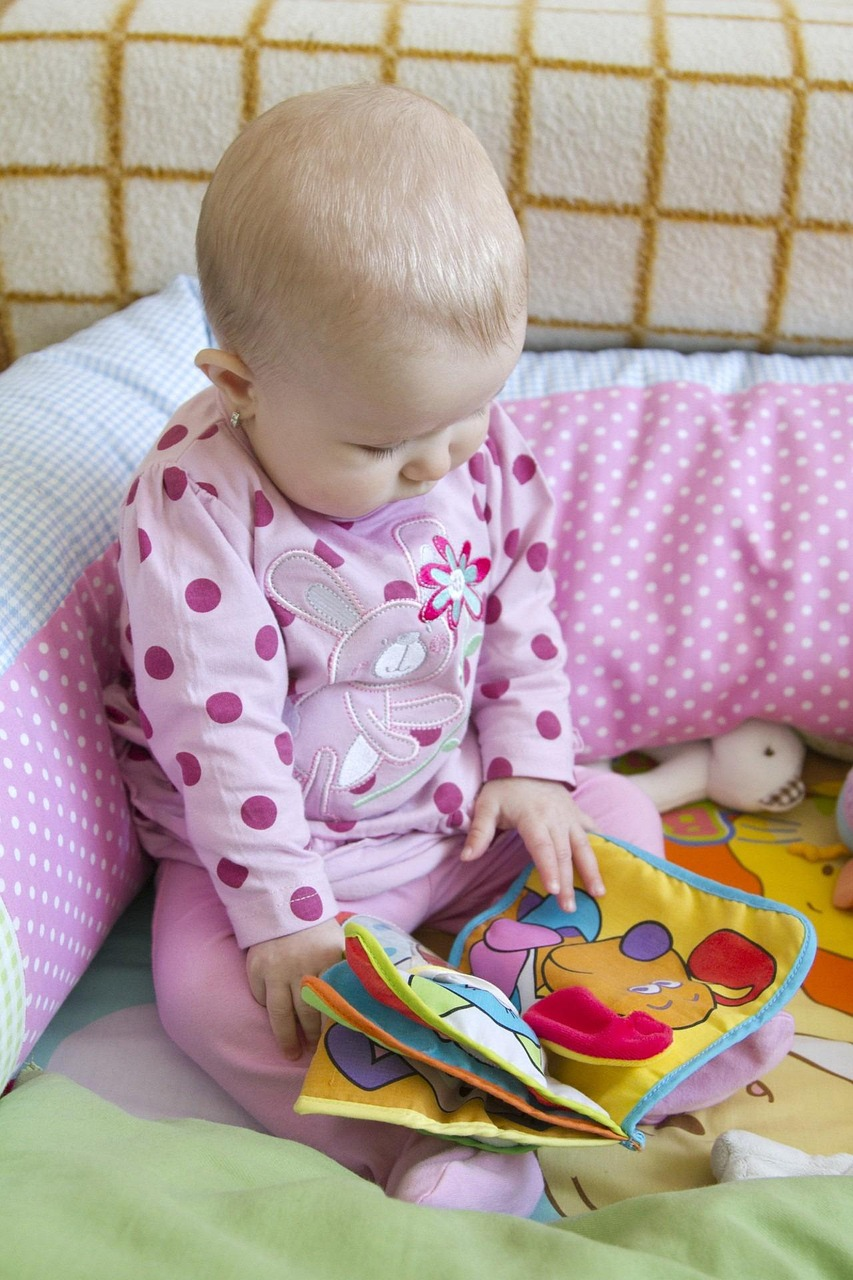
\includegraphics[width=0.62\linewidth,height=2.55cm,keepaspectratio]{media/ntp_real.png}\par\vspace{0.14cm}
      \resizebox{0.94\linewidth}{!}{%
      \begin{tikzpicture}[x=1.2cm,y=0.8cm]
        \draw[->,>=Stealth] (0,0) -- (5.5,0) node[right] {\scriptsize Confiance};
        \draw[fill=AubayTeal!35,draw=AubayTeal] (0,0.9) rectangle (4.7,1.3) node[midway] {\scriptsize\textbf{0.78}};
        \node[anchor=east] at (-0.1,1.1) {\scriptsize Vision};
        \draw[fill=gray!30,draw=gray] (0,0.1) rectangle (1.1,0.5) node[midway] {\scriptsize 0.17};
        \node[anchor=east] at (-0.1,0.3) {\scriptsize Langage};
        \draw[<->,AubaySuccess,thick] (1.1,0.3) -- (4.7,0.3) node[midway,above=-0.03cm] {\scriptsize ancrage visuel};
      \end{tikzpicture}}
    \column{0.485\textwidth}
      \centering
      {\footnotesize\itshape « The man is sitting with his legs crossed\ldots »}\par\vspace{0.08cm}
      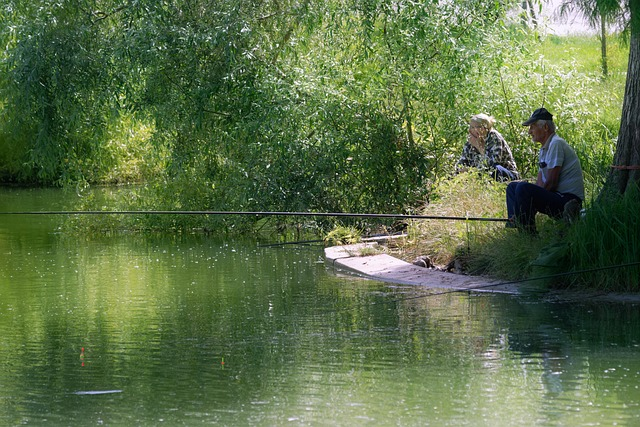
\includegraphics[width=0.62\linewidth,height=2.55cm,keepaspectratio]{media/ntp_hallu.png}\par\vspace{0.14cm}
      \resizebox{0.94\linewidth}{!}{%
      \begin{tikzpicture}[x=1.2cm,y=0.8cm]
        \draw[->,>=Stealth] (0,0) -- (5.5,0) node[right] {\scriptsize Confiance};
        \draw[fill=AubayTeal!35,draw=AubayTeal] (0,0.9) rectangle (3.5,1.3) node[midway] {\scriptsize 0.58};
        \node[anchor=east] at (-0.1,1.1) {\scriptsize Vision};
        \draw[fill=gray!30,draw=gray] (0,0.1) rectangle (3.9,0.5) node[midway] {\scriptsize\textbf{0.65}};
        \node[anchor=east] at (-0.1,0.3) {\scriptsize Langage};
        \node[text=AubayDanger,anchor=south west] at (3.0,1.45) {\scriptsize\textbf{DÉPASSEMENT}};
      \end{tikzpicture}}
  \end{columns}
\end{frame}

% ============================================================
% S08bis — Pipeline NTP (schéma papier de référence)
% ============================================================
\begin{frame}{La pipeline NTP en détail}
  \framesubtitle{Azachi et al., \textit{Leveraging NTPs for Efficient Hallucination Detection}}
  \begin{columns}[c,onlytextwidth]
    \column{0.58\textwidth}
      \centering
      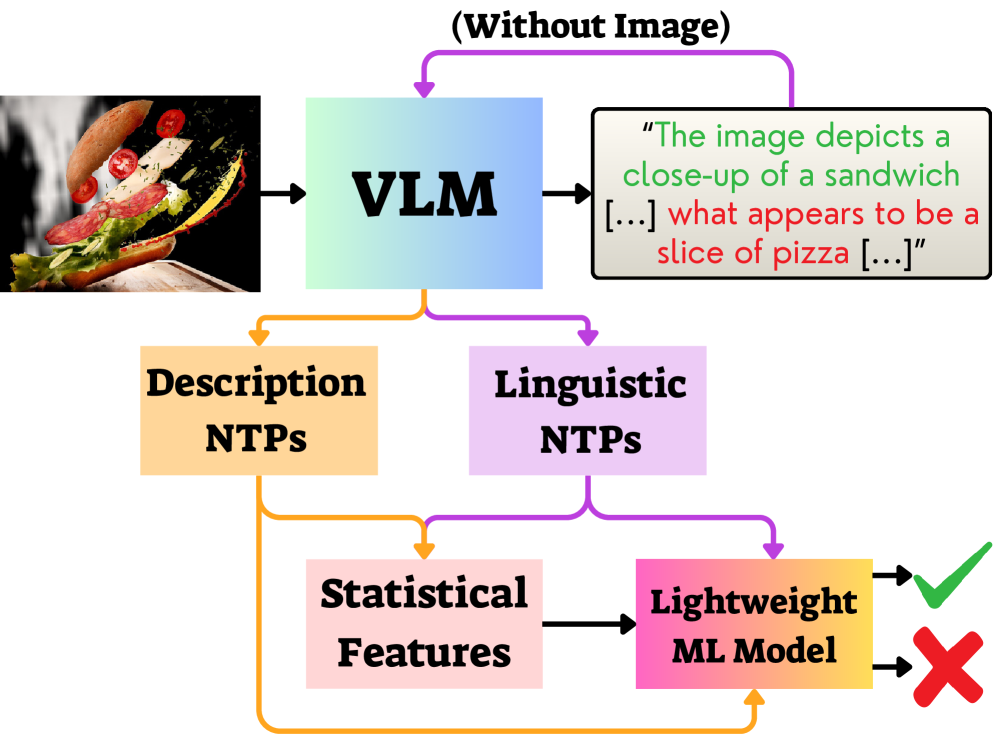
\includegraphics[width=\linewidth,height=0.78\textheight,keepaspectratio]{media/illustration_ntp.png}
    \column{0.38\textwidth}
      \AubayFocusPanel{Deux flux, un classifieur}{NTPs \textbf{avec} image vs \textbf{sans} image\\[0.35em]
      $\rightarrow$ descripteurs par phrase\\[0.35em]
      $\rightarrow$ classifieur léger.}
  \end{columns}
  \AubayTraceRef{A.1.1}
\end{frame}

% ============================================================
% S09 — Corriger : ASD
% ============================================================
\begin{frame}{Corriger : piloter les activations du modèle}
  \framesubtitle{ASD : Activation Steering Decoding}
  \begin{itemize}
    \item Calibration contrastive : tokens \textbf{factuels} \textit{vs} \textbf{hallucinés}
    \item Vecteur de contrôle injecté au \textbf{tiers central du décodeur}
    \item $\alpha$ (contraste), $\lambda$ (intensité) : \textbf{recherche manuelle}
  \end{itemize}
  \vspace{0.15cm}
  \centering
  \resizebox{0.86\linewidth}{!}{%
  \begin{tikzpicture}[
    node distance=0.95cm and 1.15cm,
    basebox/.style={rounded corners=4pt,draw=AubayInk,fill=white,minimum width=2.35cm,minimum height=0.7cm,align=center,font=\small\bfseries},
    realbox/.style={basebox,draw=AubaySuccess,fill=AubaySuccess!10},
    biasbox/.style={basebox,draw=AubayDanger,fill=AubayDanger!10},
    resultbox/.style={basebox,draw=AubayOrange,fill=AubayOrange!10},
    arrow/.style={->,>=Stealth,thick,draw=AubayInk}
  ]
    \node[basebox] (prompt) {Image + prompt};
    \node[realbox,right=1.2cm of prompt,yshift=0.8cm] (real) {Voie réalité\\$\pi^+$};
    \node[biasbox,right=1.2cm of prompt,yshift=-0.8cm] (bias) {Voie biais\\$\pi^-$};
    \node[basebox,right=1.15cm of real] (logreal) {logits réalité\\$\ell^+$};
    \node[basebox,right=1.15cm of bias] (logbias) {logits biais\\$\ell^-$};
    \node[resultbox,right=1.25cm of logreal,yshift=-0.8cm] (asd) {ASD\\logits corrigés};
    \node[resultbox,right=1.05cm of asd] (result) {texte};
    \draw[arrow] (prompt) -- (real);
    \draw[arrow] (prompt) -- (bias);
    \draw[arrow] (real) -- (logreal);
    \draw[arrow] (bias) -- (logbias);
    \draw[arrow,draw=AubayTeal] (logreal) -- node[above,font=\small\bfseries,text=AubayTeal] {$+(1+\alpha)$} (asd);
    \draw[arrow,draw=AubayDanger] (logbias) -- node[below,font=\small\bfseries,text=AubayDanger] {$-\alpha$} (asd);
    \draw[arrow] (asd) -- (result);
  \end{tikzpicture}}
  \vspace{0.22cm}

  \centering
  \begin{minipage}{0.78\textwidth}
    \AubayFocusPanel{Décodage contrastif}{$\mathrm{logit}_{ASD} = (1+\alpha)\cdot\ell^{+} - \alpha\cdot\ell^{-}$, on \textbf{soustrait le biais statistique} du modèle. Zéro réentraînement.}
  \end{minipage}
\end{frame}

% ============================================================
% S10 — Pipeline filter+asd
% ============================================================
\begin{frame}{L'architecture finale : \texttt{filter+asd}}
  \framesubtitle{Corriger uniquement quand c'est risqué}
  \centering
  \resizebox{0.88\linewidth}{!}{%
  \begin{tikzpicture}[
    box/.style={rounded corners=5pt,draw=AubayInk,fill=white,minimum width=2.35cm,minimum height=0.72cm,align=center,font=\small\bfseries},
    bluebox/.style={box,draw=AubayTeal,fill=AubayTeal!10},
    orangebox/.style={box,draw=AubayOrange,fill=AubayOrange!10},
    greenbox/.style={box,draw=AubaySuccess,fill=AubaySuccess!10},
    redbox/.style={box,draw=AubayDanger,fill=AubayDanger!10},
    graybox/.style={box,draw=AubaySlate,fill=AubayStone},
    arrow/.style={->,>=Stealth,thick,draw=AubayInk},
    softarrow/.style={->,>=Stealth,thick,dashed,draw=AubaySlate}
  ]
    \node[graybox]  (input) at (0,3.1) {Image\\+ prompt};
    \node[graybox]  (vlm)   at (2.9,3.1) {VLM\\description};
    \node[bluebox]  (split) at (5.8,3.1) {Découpage\\en phrases};
    \node[bluebox]  (ntp)   at (8.7,3.1) {NTP\\score de risque};
    \node[greenbox] (low)  at (6.8,1.75) {Risque faible\\on conserve};
    \node[redbox]   (high) at (10.6,1.75) {Risque élevé\\on corrige};
    \node[greenbox]  (kept)  at (6.8,0.55) {Phrase\\conservée};
    \node[orangebox] (asd)   at (10.6,0.55) {ASD\\réduit le biais};
    \node[greenbox]  (fixed) at (10.6,-0.65) {Phrase\\corrigée};
    \node[graybox,minimum width=3.1cm] (final) at (8.7,-1.8) {Texte final corrigé};
    \draw[arrow] (input) -- (vlm);
    \draw[arrow] (vlm) -- (split);
    \draw[arrow] (split) -- (ntp);
    \draw[softarrow,draw=AubaySuccess] (ntp.south) -- (low.north);
    \draw[softarrow,draw=AubayDanger] (ntp.south) -- (high.north);
    \draw[arrow] (low) -- (kept);
    \draw[arrow] (high) -- (asd);
    \draw[arrow] (asd) -- (fixed);
    \draw[arrow] (kept.south) |- (final.west);
    \draw[arrow] (fixed.south) |- (final.east);
    \node[draw=AubaySuccess,line width=1.6pt,rounded corners=7pt,fit=(low)(kept),inner sep=7pt,
          label={[font=\small\bfseries,text=AubaySuccess,fill=white,inner sep=2pt]west:PISTE OK}] {};
    \node[draw=AubayDanger,line width=1.6pt,rounded corners=7pt,fit=(high)(asd)(fixed),inner sep=7pt,
          label={[font=\small\bfseries,text=AubayDanger,fill=white,inner sep=2pt]east:PISTE ALERTE}] {};
  \end{tikzpicture}}
  \vspace{0.18cm}

  \centering
  \AubayStatusChip{AubayTeal}{ZERO-SHOT}\hspace{0.15cm}
  \AubayStatusChip{AubayOrange}{INTERVENTION CIBLÉE}\hspace{0.15cm}
  \AubayStatusChip{AubaySuccess}{COÛT MARGINAL QUASI NUL}
  \AubayTraceRef{A.1.5}
\end{frame}
